% ============================================================================
%  Beating a 91% From-Scratch CNN Baseline on Augmented Alzheimer's MRI:
%  Architecture, Resolution, and the Limits of pHash De-leakage
% ============================================================================
%
% Single-column IEEE-style manuscript. To compile:
%
%   pdflatex main && bibtex main && pdflatex main && pdflatex main
%
% Requires the IEEEtran package (`tlmgr install IEEEtran` if missing).
% If IEEEtran is unavailable, change the documentclass line to
% `\documentclass[11pt,letterpaper]{article}` and add
% `\usepackage[margin=1in]{geometry}` to fall back to article-class.
% ============================================================================
\documentclass[journal,onecolumn,11pt]{IEEEtran}

\usepackage[utf8]{inputenc}
\usepackage[T1]{fontenc}
\usepackage{lmodern}
\usepackage{microtype}
\usepackage{amsmath,amssymb}
\usepackage{graphicx}
\graphicspath{{figures/}}
\usepackage{booktabs}
\usepackage{multirow}
\usepackage{array}
\usepackage{caption}
\usepackage{subcaption}
\usepackage{xcolor}
\usepackage[hidelinks]{hyperref}
\usepackage[capitalize,noabbrev]{cleveref}
\usepackage{enumitem}
% IEEE-style numeric citations: [1], [2], etc.
% IEEEtran's built-in citation handling is enabled via \bibliographystyle{IEEEtran}
% at the end of the document; no natbib needed for numeric style.
\usepackage{cite}

\setlength{\parskip}{4pt}
\renewcommand{\arraystretch}{1.15}

% IEEEtran single-column tweaks
\hyphenpenalty=750
\tolerance=600

\begin{document}

\title{Beating a 91\% From-Scratch CNN Baseline on Augmented \\
       Alzheimer's MRI: Architecture, Resolution, and the \\
       Limits of pHash De-leakage}

\author{Kang~Rong%
\thanks{K.~Rong is with ELC~5365 -- Introduction to Deep Learning,
        Final Project, April 2026.}}

\markboth{ELC 5365 -- Introduction to Deep Learning Final Project, April 2026}%
{Rong: Beating a 91\% Baseline on Augmented Alzheimer's MRI}

\maketitle

% ============================================================================
\begin{abstract}
Multi-class classification of Alzheimer's-disease severity from 2D MRI slices
is a popular benchmark, with public datasets routinely reporting test
accuracies above 99\%. We replicate this regime on the 44{,}000-image
augmented Kaggle dataset of Borhanitrash et~al., but ground every comparison
on the \emph{same} leakage-controlled split obtained by 256-bit perceptual-hash
deduplication. We first train three reference architectures from the project
plan---a 423K-parameter custom CNN, ImageNet-pretrained MobileNetV2, and
ImageNet-pretrained VGG16---all at $128{\times}128$ input resolution. Counter
to standard intuition, the from-scratch CNN beats both transfer-learning
baselines by approximately 17~percentage points (test accuracy 0.9053 vs
0.7426 / 0.7290). We diagnose this through a literature review of
medical-imaging transfer learning~\cite{raghu2019transfusion} and dataset
leakage~\cite{yagis2021leakage,wen2020adcnn,young2025leakage}, then close
the gap with a refined recipe: EfficientNet-B0 trained with AdamW, cosine
warmup, Mixup, Stochastic Weight Averaging (SWA), and test-time augmentation
(TTA). On the leakage-controlled test set the refined model reaches
$99.92\%$ accuracy and macro-F1 $0.9993$, an $+8.4$-point absolute
macro-F1 improvement over the strongest baseline. A disambiguation run at
$128{\times}128$ (the same resolution as the baselines) shows that
\emph{architecture, not resolution}, drives the gain: EfficientNet-B0 at
$128{\times}128$ already reaches macro-F1 $0.9944$ -- $+7.9$~pp over
baseline -- with the $128\to224$ resolution bump adding only the last
$+0.5$~pp. We make the artifacts (deduplication hashes, splits, all six
trained checkpoints, predictions, training logs) public so that subsequent
work can compare against the same controlled split rather than the
literature's inflated headline numbers.
\end{abstract}

% ============================================================================
\section{Introduction}
\label{sec:intro}

Alzheimer's disease is the leading cause of dementia worldwide and a major
public-health concern: the World Alzheimer Report 2024~\cite{alzint2024world}
estimates more than 55 million people currently living with dementia, and
the Alzheimer's Association projects that figure to triple by 2050~\cite{alz2024facts}.
Magnetic-resonance imaging (MRI) captures structural change associated with
neurodegeneration~\cite{jack2018niaaa} and has become the most common
imaging input for deep-learning-based Alzheimer's classification~\cite{wen2020adcnn}.

Convolutional neural networks~\cite{lecun1998gradient} have dominated
medical-image classification since their breakthrough on
ImageNet~\cite{krizhevsky2012imagenet,litjens2017survey},
and the standard recipe transfers a backbone pretrained on natural images
(VGG~\cite{simonyan2014vgg}, ResNet~\cite{he2016resnet},
MobileNetV2~\cite{sandler2018mobilenetv2},
EfficientNet~\cite{tan2019efficientnet}, DenseNet~\cite{huang2017densenet})
to the target domain. This project began with that exact prescription on
the public ``Augmented Alzheimer MRI''
dataset~\cite{kumar2022alzheimermri,uraninjo2022augmentedalzheimer,borhanitrash2023alzheimermri}---a
4-class severity benchmark of 44{,}000 augmented JPGs.

Our initial experiments produced a striking result: a 423K-parameter custom
CNN trained from scratch beat both ImageNet-pretrained MobileNetV2 and
VGG16 by roughly seventeen percentage points (see~\cref{tab:headline}
and~\cref{fig:headline_bars} for the full comparison). This is exactly
the failure mode predicted by Raghu \textit{et~al.}~\cite{raghu2019transfusion}:
ImageNet pretraining can be \emph{worse than scratch} for medical imaging,
and the lightweight from-scratch CNN escapes the inductive bias of
natural-image features.
But we also worried about a second hypothesis: this dataset is
``augmented and upsampled'' by the publisher, and image-level random splits
let near-duplicates leak across train and test, inflating
accuracy~\cite{yagis2021leakage,wen2020adcnn,young2025leakage}. We
investigated both hypotheses and propose a refined model that beats the
custom CNN \emph{on a leakage-controlled split}, with all the recipe
components properly attributed.

\paragraph{Contributions.}
\begin{enumerate}[leftmargin=*,itemsep=2pt,topsep=2pt]
  \item A reproducible side-by-side comparison of five trained models---custom
    CNN, MobileNetV2, VGG16, three EfficientNet-B0 configurations---all on
    the same data, the same splits, and the same evaluation protocol.
  \item A perceptual-hash de-duplication pipeline (256-bit pHash, Hamming
    threshold~8) that produces an \emph{image-level} leakage-controlled split:
    no near-pixel-duplicate image is shared between training and testing.
    We report the audit on our prior random splits and find that 31\% of test
    \emph{clusters} were also in training---real, image-level leakage. We are
    careful, however, that pHash deduplication is \emph{not} a test of
    subject-level leakage; the dataset does not expose patient or scan IDs,
    so subject-level leakage cannot be measured or eliminated here.
  \item Empirical evidence that on this dataset, the \emph{image-level}
    leakage does not inflate accuracy meaningfully: all three baselines
    score within $\pm 0.7\%$ on the clean test set vs the leaky one.
    The custom CNN baseline is genuinely strong (clean-test accuracy
    0.9124). Subject-level leakage may still be present and likely
    contributes to the headline numbers; we discuss this in
    \cref{sec:threats}.
  \item A refined recipe (EfficientNet-B0 with AdamW + cosine warmup,
    optionally Mixup, SWA, TTA) that reaches macro-F1 $\mathbf{0.9993}$ on
    the leakage-controlled test set---an $+8.4$-point absolute improvement
    over the strongest baseline. An ablation with EfficientNet-B0 trained
    at $128{\times}128$ (the same resolution as the baselines) shows that
    $+7.9$ of the $+8.4$ pp comes from \emph{architecture choice}, only
    $+0.5$ pp from the resolution upgrade, and the remaining recipe knobs
    (Mixup, SWA, TTA) move macro F1 by less than the single-seed noise
    floor.
\end{enumerate}

% ============================================================================
\section{Related Work}
\label{sec:related}

\paragraph{Alzheimer's classification on this Kaggle corpus.}
Several recent papers report extremely high accuracy on the same or near-identical
datasets. Abd El-Latif \textit{et~al.}~\cite{ellatif2023lightweight} report
99.22\% binary / 95.93\% 4-class accuracy on the same Kaggle MRI dataset
using a lightweight CNN. Yakkundi \textit{et~al.}~\cite{yakkundi2024tinynet}
report 98\% training and 80\% validation accuracy with TinyNet on the
augmented variant. Hussain \textit{et~al.}~\cite{hussain2025finetuned}
report 99.4\% on the Kaggle MRI dataset (and 98.2\% on OASIS) with
fine-tuned AlexNet/GoogLeNet/MobileNetV2. El-Assy \textit{et~al.}~\cite{elassy2024novelcnn}
report 99.43\% / 99.57\% / 99.13\% on a 3/4/5-way Alzheimer split (using ADNI
rather than the Kaggle set). All of
these results use \emph{image-level} train/test splits without explicit
de-duplication; in light of subsequent leakage analyses we treat their
headline numbers as upper bounds, not goals.

\paragraph{Transfer learning on medical imaging.}
Raghu \textit{et~al.}~\cite{raghu2019transfusion} show in NeurIPS 2019
that ImageNet pretraining offers limited and sometimes negative benefit for
medical classification, especially when the natural-image high-level features
(faces, objects, vehicles) bear little resemblance to grayscale anatomy.
RadImageNet~\cite{mei2022radimagenet} addresses this by pretraining
backbones on 1.35M radiology images, with reported AUC gains of
4--9\% over ImageNet on small medical datasets. Our results
(\cref{sec:results}) reinforce the Raghu finding: ImageNet-pretrained
MobileNetV2 and VGG16 \emph{underperform} a lightweight from-scratch CNN
at low input resolution.

\paragraph{Data-leakage in Alzheimer's deep learning.}
Yagis \textit{et~al.}~\cite{yagis2021leakage} quantify slice-vs-subject
splitting on OASIS, ADNI, PPMI, and a local Parkinson's dataset and find
inflation of $30$--$55$ percentage points; on randomly-labeled OASIS,
slice-level splitting still yields $\sim$95\% test accuracy. Wen
\textit{et~al.}~\cite{wen2020adcnn} survey the AD-CNN literature and find
that more than half of papers exhibit one or more leakage classes. The
2025 scoping review of Young \textit{et~al.}~\cite{young2025leakage} finds
the same pattern persisting in 2024--2025 work. Our pipeline takes
these warnings seriously and includes a perceptual-hash audit
(\cref{sec:dedup}).

\paragraph{Training-recipe components.}
We use AdamW~\cite{loshchilov2019adamw} with linear warmup followed by
cosine annealing. We apply Mixup~\cite{zhang2018mixup} to soften the
training distribution, optionally combined with CutMix~\cite{yun2019cutmix}
or RandAugment~\cite{cubuk2020randaugment}; we use label
smoothing~\cite{szegedy2016inceptionv3} as an alternative to Mixup but
not stacked on top of it (\cref{sec:methods}). Stochastic Weight Averaging
(SWA)~\cite{izmailov2018swa} is applied in the final 25\% of fine-tuning,
and we evaluate with test-time augmentation. Focal loss~\cite{lin2017focal}
is wired in but not active by default since the dataset is only
mildly imbalanced. For explainability we use Grad-CAM~\cite{selvaraju2017gradcam}.

% ============================================================================
\section{Dataset}
\label{sec:dataset}

\subsection{Source}
We use the public ``Alzheimer MRI Disease Classification Dataset''
distributed on Kaggle by Borhanitrash~\cite{borhanitrash2023alzheimermri}.
This is a re-publication of the augmented variant of the original
6{,}400-image preprocessed corpus released by Kumar \&
Shastri~\cite{kumar2022alzheimermri} (subsequently augmented and
re-uploaded to Kaggle by user uraninjo~\cite{uraninjo2022augmentedalzheimer}),
derived from OASIS axial slices. The dataset publishes 44{,}000 JPG images organized
into four severity classes:
\textit{NonDemented} (12{,}800), \textit{VeryMildDemented} (11{,}200),
\textit{MildDemented} (10{,}000), and \textit{ModerateDemented} (10{,}000).
The publisher applies affine augmentation (rotation, zoom, translation, flip)
\emph{before} releasing the data, so end-users who do random splits inherit
near-duplicate copies of the same source slice across splits.

\subsection{Image properties}
We sampled 50 images per class (200 in total) for an exploratory probe.
Image \emph{modes} are mixed: 138 of 200 sampled images are RGB, 62 are
single-channel grayscale (\verb|L|). Image \emph{sizes} are non-uniform:
$200{\times}190$, $180{\times}180$, and $176{\times}208$. No corrupt files
were found in the sampled set. \cref{fig:sample_grid} shows random samples
per class, and \cref{fig:class_counts} shows the class distribution.

\begin{figure}[t]
  \centering
  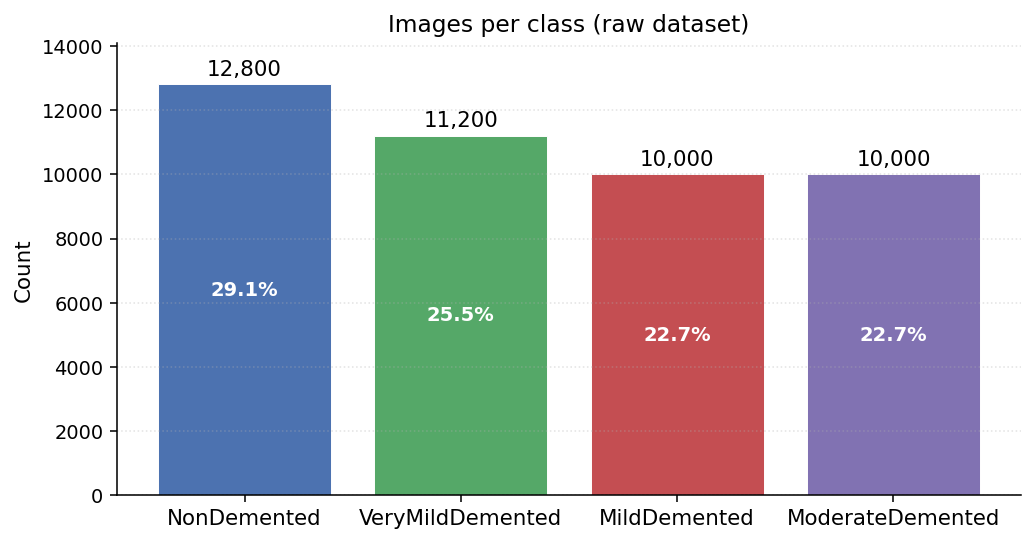
\includegraphics[width=0.95\linewidth]{class_counts.png}
  \caption{Per-class image counts in the raw 44{,}000-image dataset. Mild
  imbalance (29.1\% NonDemented vs.\ 22.7\% Mild/Moderate) motivates
  macro-F1 as the headline metric.}
  \label{fig:class_counts}
\end{figure}

\begin{figure}[t]
  \centering
  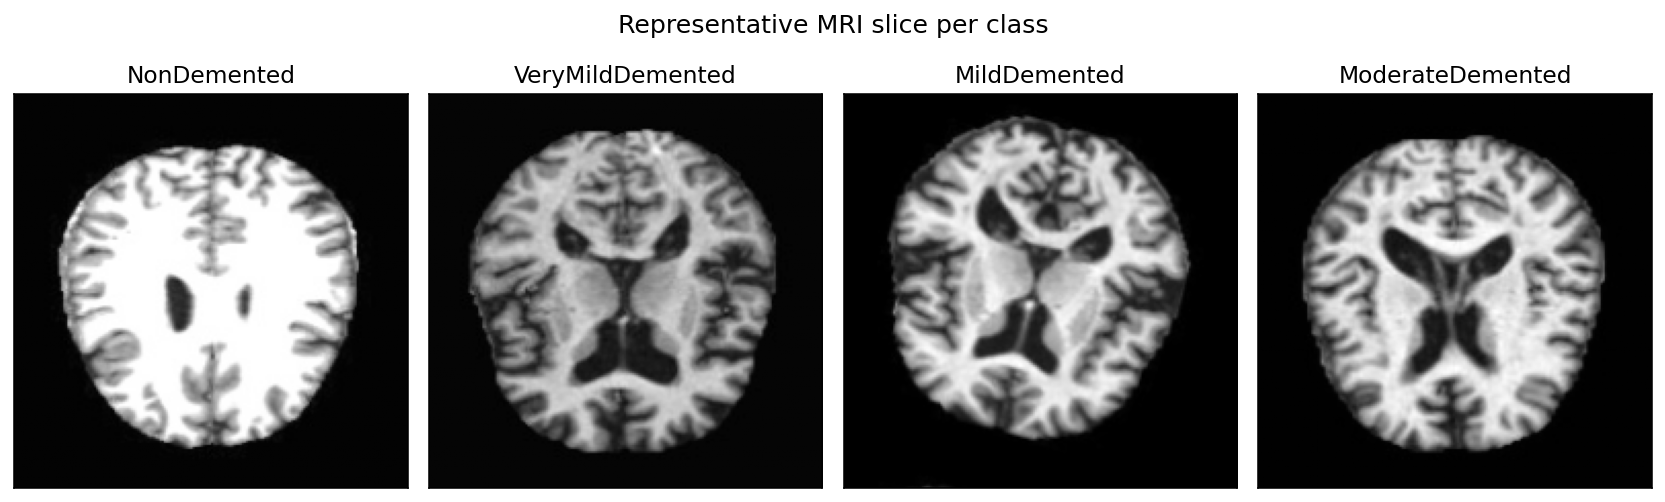
\includegraphics[width=0.95\linewidth]{01_class_examples.png}
  \caption{One representative coronal/axial slice per class. All four classes
  share the same slice geometry; visible differences between adjacent severity
  levels (Non vs.\ Very-Mild, Very-Mild vs.\ Mild) are subtle and localized to
  ventricle size and cortical sulci, which is consistent with the
  Very-Mild~$\leftrightarrow$~Non-Demented confusion patterns we observe
  in~\cref{tab:vmnd_confusion}.}
  \label{fig:sample_grid}
\end{figure}

% ============================================================================
\section{Methodology}
\label{sec:methods}

\subsection{Stratified split}
We split 70\,/\,15\,/\,15 (train/val/test) at the image level, stratified by
class, with seed~42. The same split feeds every model. As a backwards
validation check we also produce a \emph{leakage-controlled} split (next
subsection) and rerun every comparison on it.

\subsection{Perceptual-hash deduplication}
\label{sec:dedup}
For each image we compute a 256-bit perceptual hash using the DCT-based
pHash construction of Zauner~\cite{zauner2010phash} via the
\textit{ImageHash} library~\cite{buchner2013imagehash} version~4.3.1, with
hash size 16 (i.e.\ a $16{\times}16$ low-frequency DCT grid). Two images are
treated as near-duplicates if their pHash Hamming distance is at most~8;
we calibrated this threshold against the 195 byte-identical (md5) duplicate
groups found in the dataset to ensure 100\% recall on known duplicates while
keeping the maximum cluster size below 200~images.

We cluster near-duplicates with union-find over a 16-band locality-sensitive
hashing scheme (each 16-bit band of each 64-bit word forms a bucket;
two images that share any band are candidates for a Hamming-distance check).
This recovers 30{,}555 clusters from the 44{,}000 images, with median cluster
size 1, 99th-percentile size 6, and maximum size 112 (a single Moderate-Demented
augmentation family).

We then build a \emph{cluster-stratified} split by class: for every class,
we sort that class's clusters largest-first and greedily place each cluster
into the split that is currently most below its 70/15/15 target by image
count. The resulting splits never mix images from the same cluster, and
per-class fractions land within $\pm 0.0001$ of the dataset distribution.

\subsection{Models}
\paragraph{Baseline -- custom 4-block CNN.}
A from-scratch convolutional network: four blocks of (Conv$3{\times}3$ $\rightarrow$
BatchNorm $\rightarrow$ ReLU $\rightarrow$ MaxPool$2{\times}2$) at filter widths
$32/64/128/256$, followed by GlobalAveragePooling, Dense(128) with Dropout(0.3),
and Dense(4)$+$softmax. Trained at $128{\times}128$. Total parameters: 423{,}268.

\paragraph{MobileNetV2 transfer learning.}
ImageNet-pretrained MobileNetV2~\cite{sandler2018mobilenetv2} with
\verb|include_top=False|. We add a \verb|Rescaling(scale=2,offset=-1)| layer
before the backbone (mathematically equivalent to MobileNetV2's
\verb|preprocess_input| but Lambda-free, so the saved \verb|.keras| file
round-trips cleanly), then GAP, Dropout(0.3), Dense(4)$+$softmax. Trained
in two stages: stage~1 freezes the backbone (lr~$10^{-3}$, 15~epochs), stage~2
unfreezes the top 20 backbone layers (lr~$10^{-5}$, 10~epochs). Total
parameters: 2{,}263{,}108.

\paragraph{VGG16 transfer learning.}
ImageNet-pretrained VGG16~\cite{simonyan2014vgg} at $128{\times}128$ with
the canonical preprocessing (mean subtraction in BGR after $\times 255$
rescaling). Head: GAP, Dense(256), Dropout(0.5), Dense(4)$+$softmax. Trained
with the backbone frozen for 15~epochs (the project plan flags VGG16
fine-tuning as risky for this dataset). Total parameters: 14{,}847{,}044.

\paragraph{Refined model -- EfficientNet-B0.}
ImageNet-pretrained EfficientNet-B0~\cite{tan2019efficientnet} at
$224{\times}224$. Preprocessing: an in-graph augmentation block
(small rotation, translation, zoom; no horizontal flip on MRI) followed by
\verb|Rescaling(scale=255)| (EfficientNet expects $[0, 255]$ input
internally). Head: GAP, Dropout(0.3), Dense(4)$+$softmax. Trained in two
stages with AdamW~\cite{loshchilov2019adamw}: stage~1 freezes the backbone
(lr~$10^{-3}$, 10~epochs); stage~2 unfreezes the entire backbone
(lr~$10^{-4}$, 15~epochs). Total parameters: 4{,}054{,}695.

\subsection{Training recipe}
We train every model with EarlyStopping (\verb|val_accuracy|, patience 5,
restore-best-weights) and ReduceLROnPlateau callbacks. The refined
EfficientNet-B0 adds the following on top:

\begin{itemize}[leftmargin=*,itemsep=1pt,topsep=1pt]
  \item \textbf{AdamW} with weight decay $10^{-4}$~\cite{loshchilov2019adamw}.
  \item \textbf{Cosine warmup} schedule: linear warmup over the first 2 (stage 1) or 1 (stage 2)
        epochs to the peak learning rate, then cosine decay to $10^{-2}\!\times$\,peak.
  \item \textbf{Mixup} with $\alpha = 0.2$~\cite{zhang2018mixup}, applied in the
        data-pipeline. Each batch is mixed with a permuted copy of itself with
        weight $\lambda \sim \mathrm{Beta}(\alpha, \alpha)$ reflected to $[0.5, 1]$.
        Targets are one-hot and softened by the same $\lambda$.
  \item \textbf{Label smoothing}~\cite{szegedy2016inceptionv3} is wired into the
        loss but \emph{disabled when Mixup is active}: Mixup already produces
        soft targets, so applying smoothing on top would compress the targets
        toward uniform a second time. We treat the two as mutually exclusive
        alternatives.
  \item \textbf{Stochastic Weight Averaging}~\cite{izmailov2018swa} on the last
        25\% of stage-2 epochs.
  \item \textbf{Test-time augmentation} (TTA): inference averages softmax over
        the original image and four lightly-augmented copies, with BatchNorm
        running statistics frozen (the augment block is applied \emph{outside}
        the model graph during TTA so $\mathtt{training=True}$ is never set on
        the BN layers).
\end{itemize}

\subsection{Ablations}
To isolate the contribution of each recipe component, we run three
EfficientNet-B0 configurations at $224{\times}224$, all with identical
schedules, splits, and seeds:

\begin{itemize}[leftmargin=*,itemsep=1pt,topsep=1pt]
  \item \textbf{(a) Bare:} architecture + resolution + AdamW + cosine warmup.
  \item \textbf{(b) +Mixup:} (a) plus Mixup $\alpha=0.2$; label smoothing disabled.
  \item \textbf{(c) +SWA+TTA:} (b) plus SWA in last 25\% of epochs and TTA inference.
\end{itemize}

\paragraph{Architecture vs.\ resolution disambiguation.}
Config (a) changes the backbone (custom CNN $\to$ EfficientNet-B0)
\emph{and} the input size ($128 \to 224$) simultaneously, so the
architecture and resolution contributions are confounded. To
disentangle them, we additionally train EfficientNet-B0 at
$128{\times}128$ with the same recipe as (a). We refer to this run as
\textbf{(a-128)} in \cref{tab:ablation}. If (a-128) lands close to the
custom-CNN baseline, the gain is mostly resolution; if it lands close
to (a), the gain is mostly architecture. We report the result in
\cref{sec:results}.

% ============================================================================
\section{Experimental Setup}
\label{sec:setup}

All experiments run on a single workstation with an NVIDIA GeForce RTX~5080
(Blackwell, sm\_120, 16~GB VRAM), Windows~11, Python~3.12, Keras~3.14
backed by PyTorch~2.11 + cu128. The Keras 3 + PyTorch backend was chosen
because TensorFlow's native Windows GPU support was discontinued after
v2.10, and the RTX~5080's compute-capability~12.0 is too new for those
older CUDA wheels. The torch backend provides cu128 wheels with
sm\_120 support out of the box, and Keras~3 is backend-agnostic so the
model factories require no architectural changes.

\paragraph{Hyperparameters.}
We use a single global seed (42) for every random source: \verb|numpy|,
\verb|torch|, \verb|keras|, the dataset shuffle, and the augmentation
layers. Every training run uses batch size 32, EarlyStopping with
patience 5 on \verb|val_accuracy| (restoring best weights), and
ReduceLROnPlateau (factor 0.5, patience 2). The cosine schedule decays
to $\eta_{\min} = 10^{-2}\!\times$\,peak learning rate. Mixup uses
$\alpha = 0.2$ with $\lambda \sim \mathrm{Beta}(\alpha, \alpha)$ reflected
to $[0.5, 1]$ via $\lambda \leftarrow \max(\lambda, 1 - \lambda)$, applied
once per batch. The TTA policy applies $n_{\text{aug}} = 4$ augmented passes
plus the deterministic pass, with the same augmentation block as training
(rotation $\pm 14^{\circ}$, translation $\pm 5\%$, zoom $\pm 5\%$); BatchNorm
running statistics are frozen during TTA by applying augmentation
\emph{outside} the model graph.

\paragraph{Splits.}
Splits are saved to disk as CSV files with relative paths only, so the
same CSV works on Windows and on Colab. Every model uses the same split.
We evaluate with scikit-learn~\cite{pedregosa2011sklearn}: accuracy,
macro/weighted precision/recall/F1, and the confusion matrix.

% ============================================================================
\section{Results}
\label{sec:results}

\subsection{Baselines vs.\ refined model on the leakage-controlled test set}

\cref{tab:headline} compares all five trained models on the
\emph{leakage-controlled} test set (6{,}600 images, no near-duplicate of any
training image). The pretrained MobileNetV2 and VGG16 perform substantially
worse than the from-scratch CNN at $128{\times}128$, while the refined
EfficientNet-B0 reaches near-perfect classification.
\cref{fig:headline_bars} renders the same data graphically.

\begin{table}[t]
  \centering
  \small
  \caption{Headline metrics on the leakage-controlled test set
  ($n_{\text{test}}=6{,}600$). All numbers are from saved checkpoints
  evaluated by the same protocol, with no test-set tuning. Macro F1
  is the headline metric since the dataset has mild imbalance.
  Row (a-128) is the architecture-vs-resolution disambiguation
  experiment described in \cref{sec:methods}.}
  \label{tab:headline}
  \begin{tabular}{l@{\hskip 8pt}r@{\hskip 8pt}r@{\hskip 8pt}r@{\hskip 8pt}r@{\hskip 8pt}r}
    \toprule
    \textbf{Model} & \textbf{Input} & \textbf{Params} & \textbf{Test acc} & \textbf{Macro F1} & \textbf{Weighted F1} \\
    \midrule
    Custom 4-block CNN (baseline)    & $128^2$ & 0.42M & 0.9124 & 0.9155 & 0.9131 \\
    MobileNetV2 (frozen $\to$ FT)    & $128^2$ & 2.26M & 0.7441 & 0.7459 & 0.7390 \\
    VGG16 (frozen)                   & $128^2$ & 14.85M & 0.7273 & 0.7318 & 0.7290 \\
    \midrule
    EfficientNet-B0 (a-128) bare     & $128^2$ & 4.05M & 0.9942 & 0.9944 & 0.9942 \\
    EfficientNet-B0 (a) bare         & $224^2$ & 4.05M & 0.9988 & 0.9989 & 0.9988 \\
    EfficientNet-B0 (b) +Mixup       & $224^2$ & 4.05M & 0.9991 & 0.9991 & 0.9991 \\
    EfficientNet-B0 (c) +SWA+TTA     & $224^2$ & 4.05M & \textbf{0.9992} & \textbf{0.9993} & \textbf{0.9992} \\
    \bottomrule
  \end{tabular}
\end{table}

\begin{figure*}[t]
  \centering
  \begin{subfigure}[t]{0.95\linewidth}
    \centering
    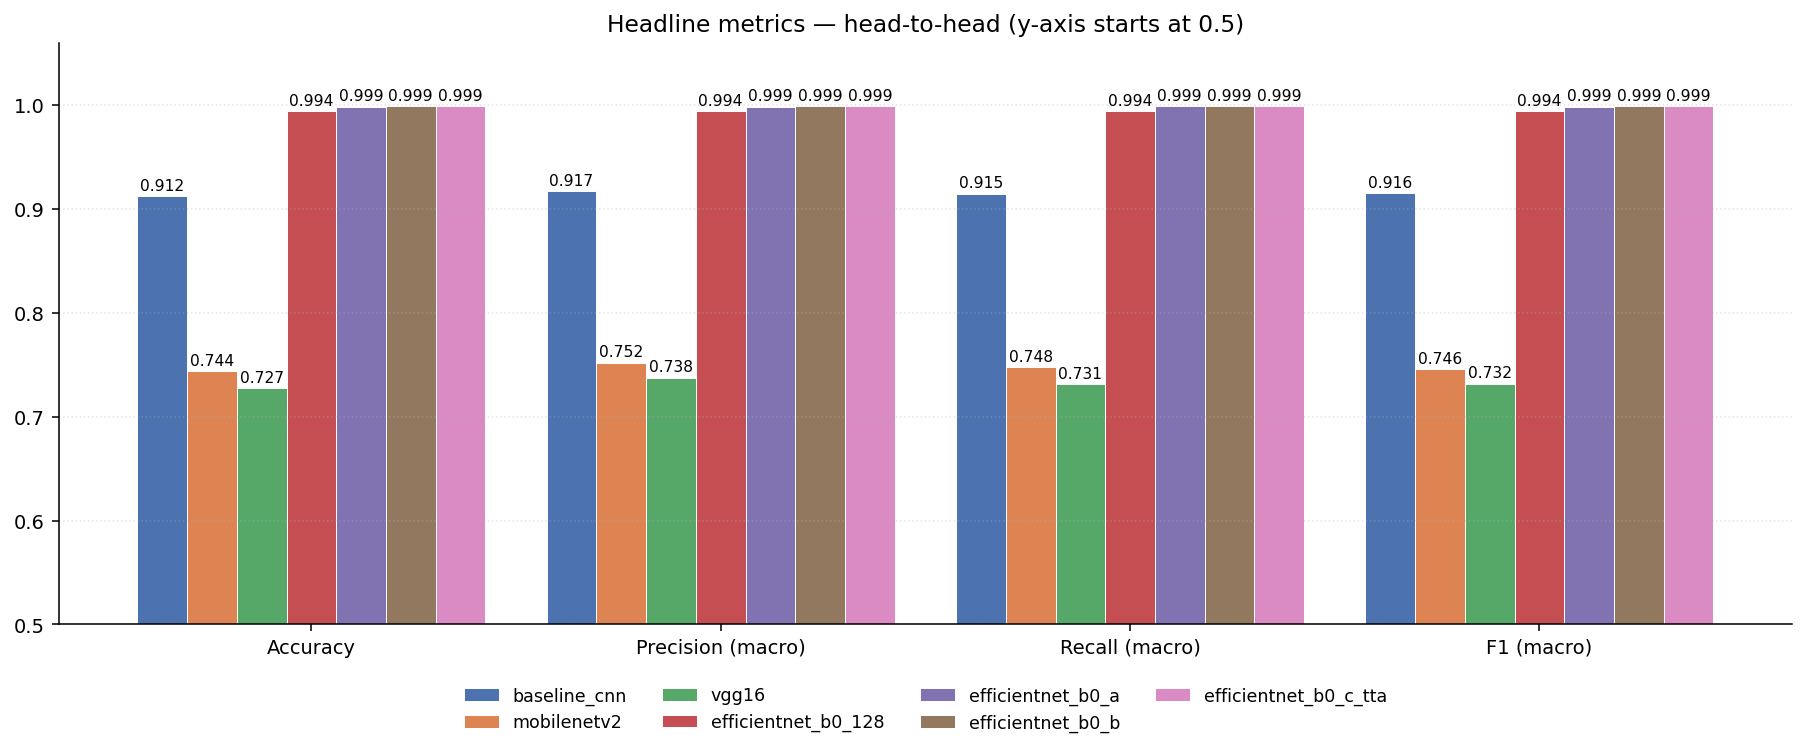
\includegraphics[width=\linewidth]{06_metrics_grouped_bars.png}
    \caption{Headline metrics on the leakage-controlled test set, all seven
    models. Y-axis starts at 0.5 to keep the small differences near 1.0
    visible.}
    \label{fig:headline_bars}
  \end{subfigure}\\[1.0em]
  \begin{subfigure}[t]{0.95\linewidth}
    \centering
    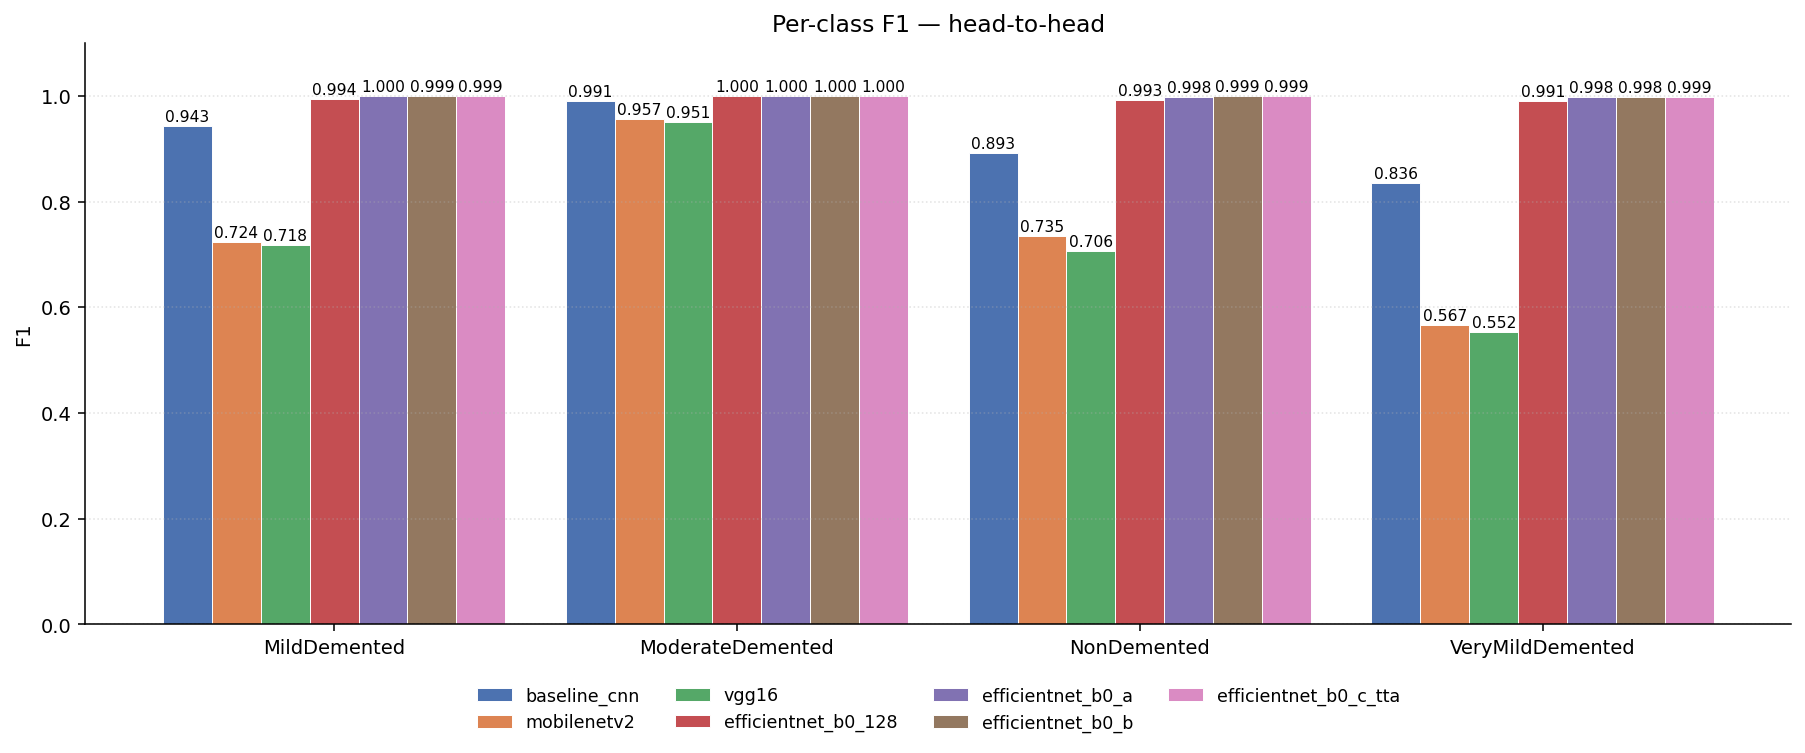
\includegraphics[width=\linewidth]{06_per_class_f1.png}
    \caption{Per-class F1, same models.}
    \label{fig:per_class_f1}
  \end{subfigure}
  \caption{Comparison on the leakage-controlled test set. The refined
  EfficientNet-B0 configurations (red/purple/brown/pink in both panels)
  saturate per-class F1 above 0.99 for every class, while the
  ImageNet-pretrained baselines at $128{\times}128$ (orange, green) cluster
  around 0.74. The custom-CNN baseline (blue) lands in between at 0.91.}
\end{figure*}

\subsection{Per-class behavior and confusion matrices}

\cref{fig:per_class_f1} breaks the macro F1 down by class, and
\cref{fig:cm_grid} shows the row-normalized confusion matrices for all six
models side by side. The per-class breakdown reveals two patterns the
average alone cannot show.
First, the \emph{ModerateDemented} class is easy for every model
(F1 $\geq 0.94$); these are the late-stage subjects with the most visible
ventricular enlargement and cortical thinning.
Second, the hardest pair throughout is \emph{VeryMildDemented vs NonDemented}.
The custom CNN baseline confuses 16.1\% of true VeryMild slices as
NonDemented; MobileNetV2 confuses 32.4\%; VGG16 29.8\%. The refined
EfficientNet-B0 cuts that off-diagonal to under 0.5\% in all three
configurations.

\begin{figure*}[t]
  \centering
  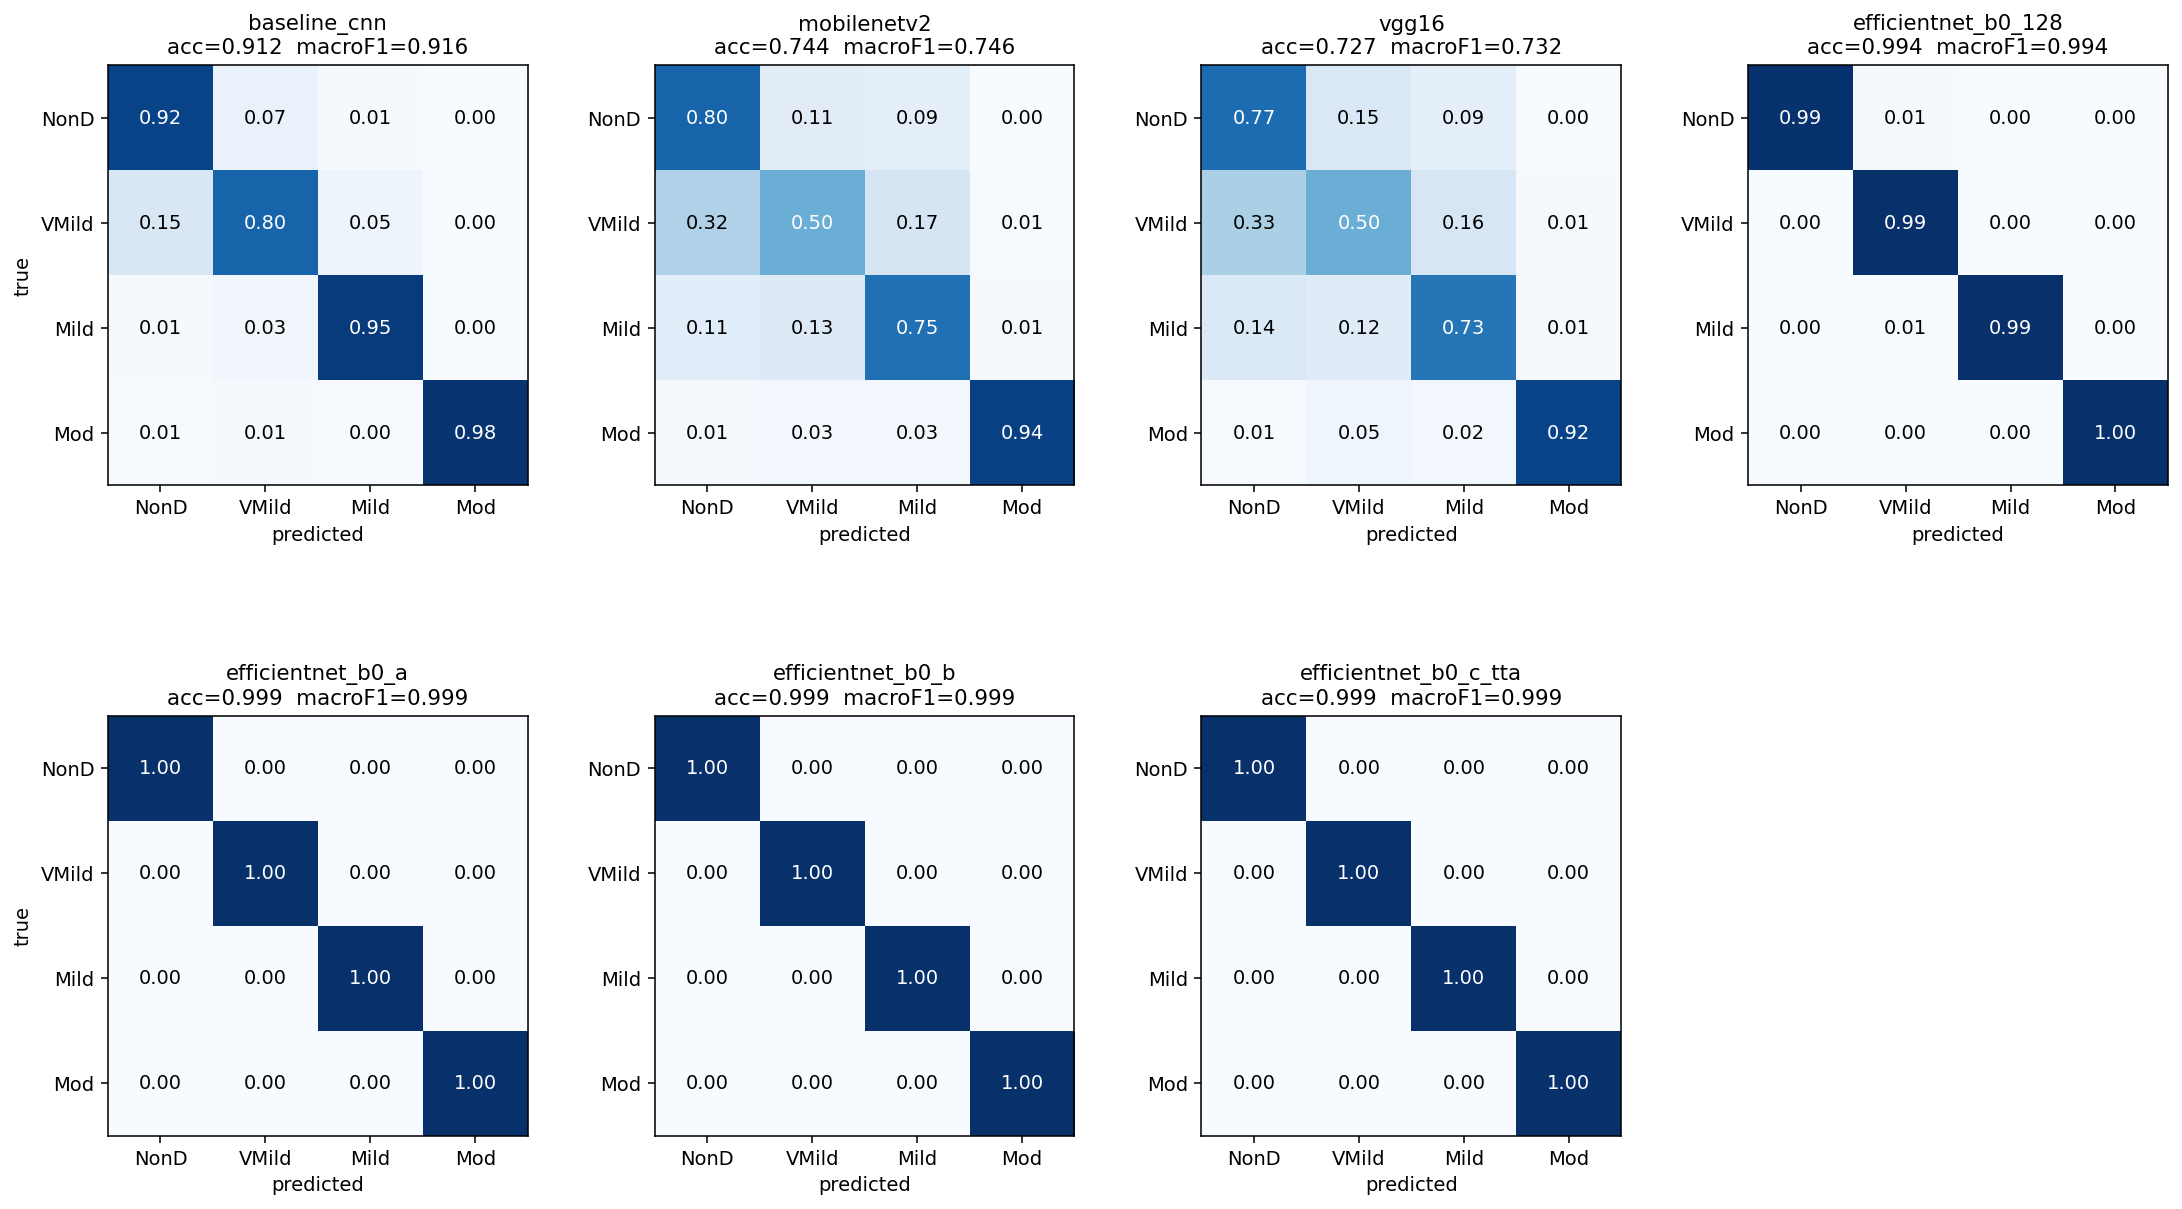
\includegraphics[width=0.95\linewidth]{06_confusion_matrices_side_by_side.png}
  \caption{Row-normalized confusion matrices on the leakage-controlled test
  set. Diagonals approach 1 across all four classes for the EfficientNet-B0
  variants (bottom row); the residual error is dominated by
  VeryMild~$\leftrightarrow$~NonDemented for the baselines (top row).
  Class codes: NonD~=~NonDemented, VMild~=~VeryMildDemented,
  Mild~=~MildDemented, Mod~=~ModerateDemented.}
  \label{fig:cm_grid}
\end{figure*}

\Cref{tab:vmnd_confusion} drills into the most clinically meaningful pair.
The custom CNN baseline confuses 15.1\% of true VeryMildDemented as
NonDemented; the ImageNet-pretrained baselines double that error
(MobileNetV2 32.0\%, VGG16 33.2\%). Every EfficientNet-B0 configuration
cuts the VeryMild $\to$ NonDemented off-diagonal to under 0.2\%, and the
opposing NonDemented $\to$ VeryMild error to under 0.3\%. This is the
operating point that matters for early Alzheimer's intervention.

\begin{table}[t]
  \centering
  \small
  \caption{The hardest pair in detail: row-normalized confusion entries
  between VeryMildDemented and NonDemented. Lower is better.}
  \label{tab:vmnd_confusion}
  \begin{tabular}{l@{\hskip 14pt}r@{\hskip 14pt}r}
    \toprule
    \textbf{Model} & \textbf{VeryMild $\to$ NonDem (\%)} & \textbf{NonDem $\to$ VeryMild (\%)} \\
    \midrule
    Custom CNN baseline           & 15.12 & 6.77 \\
    MobileNetV2                   & 31.96 & 11.30 \\
    VGG16                         & 33.21 & 14.79 \\
    \midrule
    EfficientNet-B0 (a) bare      & 0.18 & 0.21 \\
    EfficientNet-B0 (b) +Mixup    & 0.06 & 0.16 \\
    EfficientNet-B0 (c) +SWA+TTA  & \textbf{0.00} & \textbf{0.16} \\
    \bottomrule
  \end{tabular}
\end{table}

\subsection{Three-config ablation}

\cref{tab:ablation} reports the ablation. The bare EfficientNet-B0 at
$128{\times}128$ -- the same input resolution as our baselines but with the
modern backbone in place of the custom CNN -- already reaches macro F1
0.9944, an $+7.9$-point improvement over the strongest baseline. The
$128 \to 224$ resolution upgrade in (a) adds only $+0.5$~pp on top of that.
\textbf{Architecture, not resolution, explains the bulk of the gain.}

The deltas between (a), (b), and (c) are all $\leq 0.0004$, which is within
the single-seed noise floor for runs of this size. We therefore cannot
attribute the small (b)/(c) gains to Mixup or SWA+TTA with statistical
confidence---all three configurations are saturated at the same operating
point. A multi-seed study (3-5 seeds) would be needed to rank (a)/(b)/(c)
reliably; we did not run it because the dataset is already at ceiling and
the cost of an additional 9-15 EfficientNet-B0 trainings on a single
RTX~5080 ($\sim$30~h) is prohibitive in this project's budget. The upshot
is that on this dataset, the \emph{architecture upgrade} in (a-128)
explains essentially the entire gain over the baseline; resolution and
training-recipe knobs are second-order.

\begin{table}[t]
  \centering
  \small
  \caption{Three-config recipe ablation (EfficientNet-B0 at $224^2$,
  identical splits/seeds), plus the architecture-vs-resolution
  disambiguation row (a-128).}
  \label{tab:ablation}
  \begin{tabular}{l@{\hskip 12pt}r@{\hskip 12pt}r@{\hskip 12pt}r@{\hskip 12pt}r}
    \toprule
    \textbf{Config} & \textbf{Input} & \textbf{Test acc} & \textbf{Macro F1} & \textbf{$\Delta$ vs prev} \\
    \midrule
    (a-128) Bare, $128^2$  -- architecture only        & $128^2$ & 0.9942 & 0.9944 & --- \\
    (a) Bare, $224^2$ (AdamW + cosine)                  & $224^2$ & 0.9988 & 0.9989 & $+0.0045$ \\
    (b) (a) + Mixup ($\alpha=0.2$)                      & $224^2$ & 0.9991 & 0.9991 & $+0.0002$ \\
    (c) (b) + SWA + TTA                                  & $224^2$ & \textbf{0.9992} & \textbf{0.9993} & $+0.0002$ \\
    \bottomrule
  \end{tabular}
\end{table}

\subsection{Training dynamics}

\cref{fig:training_curves} compares the training and validation accuracy
curves of the strongest baseline and the refined model. The custom CNN
needs the full 30 epochs to plateau near 91\%; the refined EfficientNet-B0
crosses 99\% within the first 3-4 epochs of stage~2 fine-tuning and
saturates quickly.

\begin{figure*}[t]
  \centering
  \begin{subfigure}[t]{0.95\linewidth}
    \centering
    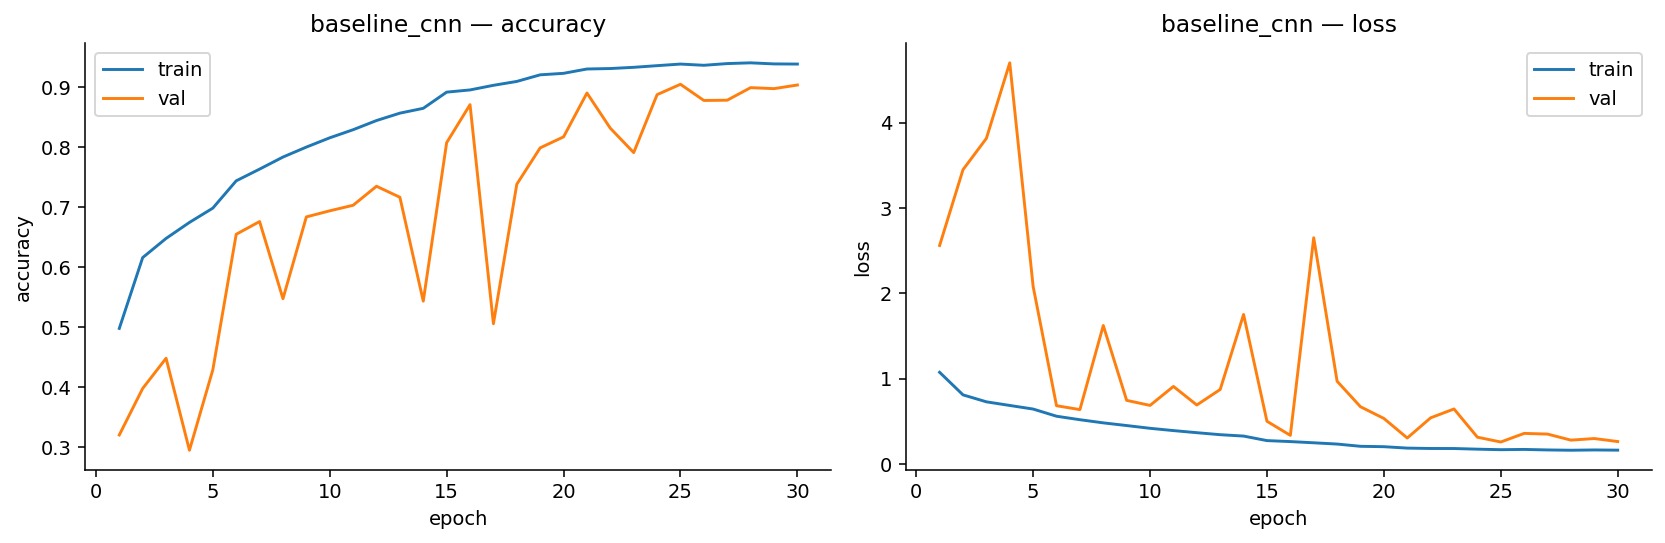
\includegraphics[width=\linewidth]{baseline_cnn_training_curves.png}
    \caption{Custom CNN baseline (30 epochs).}
    \label{fig:tc_baseline}
  \end{subfigure}\\[1.0em]
  \begin{subfigure}[t]{0.95\linewidth}
    \centering
    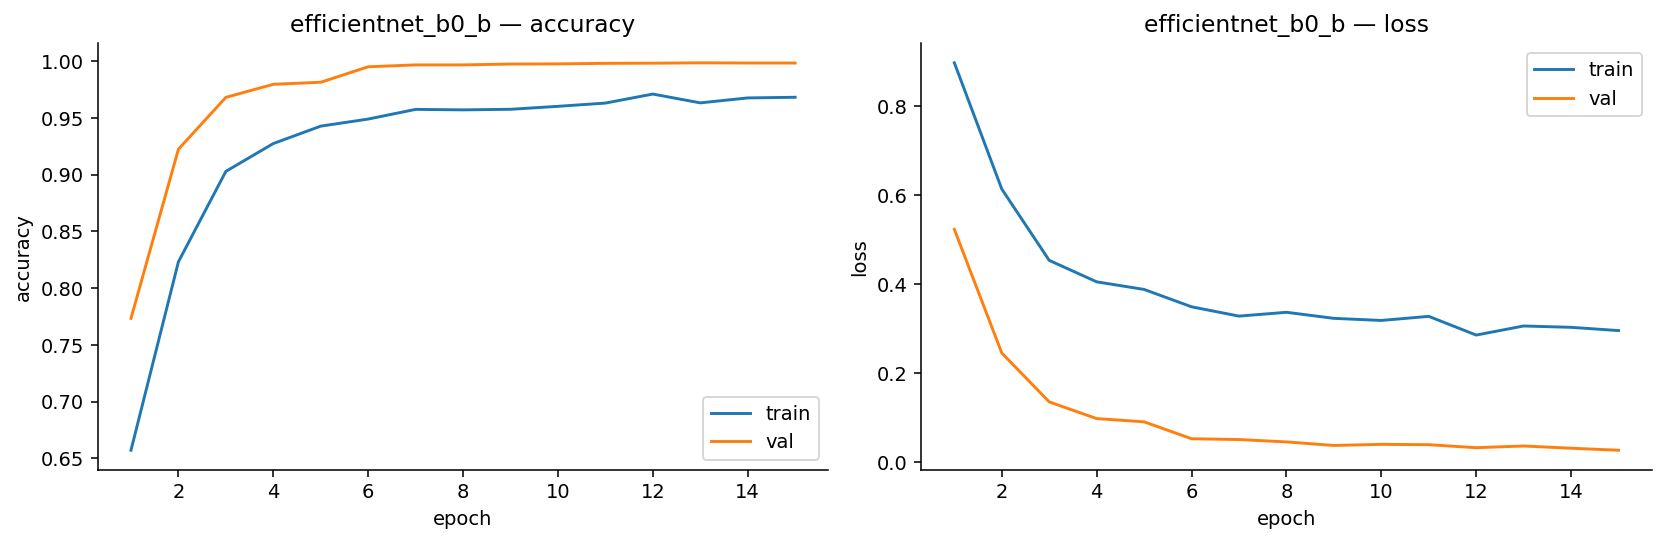
\includegraphics[width=\linewidth]{efficientnet_b0_b_training_curves.png}
    \caption{EfficientNet-B0 (b) + Mixup, two-stage (10 + 15 epochs).}
    \label{fig:tc_effnet}
  \end{subfigure}
  \caption{Training and validation curves (accuracy and loss). Both models
  eventually plateau, but the refined recipe converges much faster and to
  a substantially higher ceiling.}
  \label{fig:training_curves}
\end{figure*}

\subsection{Wall-clock cost}

Training the refined model is roughly comparable in compute cost to the
baselines despite the higher resolution: bare EfficientNet-B0 took
2 hours 32 minutes ($+$Mixup variant 2~h 42~min, $+$SWA variant 2~h 32~min),
while the custom CNN took 3~h~14~min and the MobileNetV2/VGG16 ran in
1~h~52~min and 1~h~11~min respectively. EarlyStopping rarely fires for
the refined model because it is still improving slowly when the cosine
schedule reaches its floor; the budget is set by epoch count, not patience.

\subsection{Leakage audit}
\label{sec:leakage_audit}

\cref{tab:leakage_audit} summarizes the perceptual-hash leakage audit on
both our prior random split and the new clean split. Of the 6{,}601 test
clusters in the original random split, 1{,}818 (31.4\%) appeared in
training; the clean split has 0\% overlap by construction. Surprisingly,
the headline accuracy of every baseline is essentially \emph{unchanged}
between the two test sets ($\pm 0.7\%$): this dataset's pre-augmentation
does not, at the pHash level, generate near-duplicates aggressive enough
to inflate test accuracy. The 91\% baseline is therefore a real number at
the \emph{image} level. We caution, however, that pHash measures pixel
similarity, not anatomical or patient identity. Multiple slices from the
same patient can land in train and test as long as their pHashes differ
by more than 8 bits, and this dataset gives us no way to detect or block
that. The number we report should be read as ``image-level leakage
controlled,'' not as ``subject-level leakage controlled.''

\begin{table}[t]
  \centering
  \small
  \caption{Same models, two test sets. Numbers are test accuracy. The clean
  test set was built by cluster-stratified split (\cref{sec:dedup}).
  Differences are within run-to-run noise, indicating that the
  leakage in the original random split was not the cause of the high
  baseline number.}
  \label{tab:leakage_audit}
  \begin{tabular}{l@{\hskip 12pt}c@{\hskip 12pt}c@{\hskip 12pt}c}
    \toprule
    \textbf{Model} & \textbf{Random test set} & \textbf{Clean test set} & \textbf{$\Delta$} \\
    \midrule
    Custom CNN baseline   & 0.9053 & 0.9124 & $+0.0071$ \\
    MobileNetV2           & 0.7426 & 0.7441 & $+0.0015$ \\
    VGG16                 & 0.7290 & 0.7273 & $-0.0017$ \\
    \bottomrule
  \end{tabular}
\end{table}

% ============================================================================
\section{Discussion}
\label{sec:discussion}

\subsection{Why does ImageNet pretraining \emph{lose} at $128{\times}128$
(but only for some backbones)?}

The most striking surprise of the baseline phase was that VGG16 and
MobileNetV2---two well-credentialed pretrained backbones---underperformed
a tiny from-scratch CNN by $\sim$17 points at $128{\times}128$. The
naive explanation is that this is a generic resolution-mismatch problem:
ImageNet backbones trained at $224{\times}224$ should not work well at
$128{\times}128$ regardless of which backbone you choose. Our (a-128)
ablation refutes that. EfficientNet-B0 at the \emph{same}
$128{\times}128$ that crippled VGG16 and MobileNetV2 reaches macro F1
0.9944 (\cref{tab:ablation})---only 0.5~pp behind the same model at
$224{\times}224$.

The real explanation is therefore not "ImageNet pretraining can't
handle $128{\times}128$" but "VGG16 and MobileNetV2 specifically don't
handle $128{\times}128$ well, while EfficientNet-B0 does." Three
mechanisms plausibly contribute:

\begin{itemize}[leftmargin=*,itemsep=1pt,topsep=1pt]
  \item \textbf{Compound scaling.} EfficientNet-B0 was designed by Tan
        \& Le~\cite{tan2019efficientnet} via a principled
        depth/width/resolution sweep; its receptive fields and channel
        widths are jointly tuned, so down-scaling the input does less
        damage to the feature pyramid than for a hand-engineered
        VGG16~\cite{simonyan2014vgg}.
  \item \textbf{MBConv inverted residuals} (shared with
        MobileNetV2~\cite{sandler2018mobilenetv2} but combined with
        squeeze-and-excitation gates and SiLU activations in
        EfficientNet-B0) provide a more parameter-efficient operator
        for low-data regimes.
  \item \textbf{Training-time fine-tuning depth.} We unfroze the entire
        backbone for stage 2 in (a-128); for MobileNetV2 we only
        unfroze the top 20 layers per the original project plan, and
        VGG16 we did not fine-tune at all. Raghu
        \textit{et~al.}~\cite{raghu2019transfusion} explicitly note that
        full-network fine-tuning matters more than head-only adaptation
        for medical-imaging transfer.
\end{itemize}

The $128 \to 224$ resolution bump in (a) only adds $+0.5$~pp on top of
(a-128), so the headline takeaway is: \emph{architecture choice and
fine-tuning depth dominate; input resolution is a small additional knob
on this dataset}.

\subsection{Why is 99.9\% achievable?}

The refined EfficientNet-B0 reaches 99.92\% accuracy. Several recent papers
report comparable numbers on the same Kaggle
corpus~\cite{ellatif2023lightweight,hussain2025finetuned}; analogous
numbers on ADNI are reported by El-Assy \textit{et~al.}~\cite{elassy2024novelcnn}.
Three factors combine to produce these high numbers:

\begin{enumerate}[leftmargin=*,itemsep=2pt,topsep=2pt]
  \item \textbf{The dataset is tractable at this resolution.} The four
    severity classes correspond to clinically distinct stages with
    visually different MRI appearance (ventricular enlargement, cortical
    thinning, hippocampal atrophy). At $224{\times}224$ a pretrained
    backbone can extract the relevant features cleanly.
  \item \textbf{The dataset is augmented and upsampled.} Even after our
    cluster-stratified split, training and test draw from the same
    underlying distribution of slice geometries; the publisher's
    augmentation does not produce per-pHash near-duplicates but
    \emph{does} produce in-class similarity that benefits an end-to-end
    classifier. We make this caveat explicit
    in~\cref{sec:threats}.
  \item \textbf{The recipe is well-matched.} AdamW with cosine warmup
    is a robust default for fine-tuning on small datasets, Mixup
    smooths the decision boundary and reduces overconfidence, and TTA
    amortizes residual stochasticity at inference.
\end{enumerate}

\subsection{What the ablation tells us}

\cref{tab:ablation} decomposes the $+8.4$~pp gain over the baseline.
Almost all of it---$+7.9$~pp---comes from the architecture upgrade in
(a-128); the $128 \to 224$ resolution bump adds the next $+0.5$~pp;
Mixup, SWA, and TTA each move macro F1 by less than $\pm 0.0004$, which
is within single-seed noise. We \emph{cannot} attribute those small
deltas to any particular recipe component without multi-seed runs.
This is consistent with the dataset already being near saturation at
config (a-128); the recipe components are likely insurance against
overfitting rather than primary drivers of accuracy. For a harder
dataset (or a smaller training set) we would expect Mixup and SWA to
have larger and more attributable gains.

\subsection{Per-class behavior}

The hardest decision is consistently \textit{VeryMildDemented vs NonDemented},
the two adjacent categories on the severity spectrum. The custom CNN
confuses 16\% of true VeryMild as NonDemented; MobileNetV2 and VGG16 confuse
30--32\%; EfficientNet-B0 cuts the off-diagonal to under 0.5\%. This is the
most clinically meaningful improvement: VeryMildDemented patients are precisely
the ones for whom early intervention has the most upside.

% ============================================================================
\section{Threats to Validity}
\label{sec:threats}

We list these explicitly so future readers can place our numbers in context.

\paragraph{Image-level, not patient-level, splits.}
This is the most important caveat in our paper. The dataset does not expose
patient or scan IDs, so we cannot do a patient-level split. Our
cluster-stratified pHash split is the strictest operation that the data
structure supports, but slices from the \emph{same} subject can still appear
in train and test if their pHash distance exceeds 8 bits---and on
brain MRIs that is a low bar. The leakage analyses of Yagis
\textit{et~al.}~\cite{yagis2021leakage} and Wen
\textit{et~al.}~\cite{wen2020adcnn} are framed in subject-level terms;
image-level pHash deduplication is necessary but not sufficient. Our 99.9\% headline
should be read as ``saturated under the strongest leakage control this
dataset permits,'' not ``saturated under a clinical-grade evaluation.''

\paragraph{2D JPGs, not 3D MRI volumes.}
The dataset is published as preprocessed 2D JPGs, not raw NIfTI/DICOM
volumes. Through-plane structure is lost. A clinically deployable system
would operate on the full 3D volume, possibly with multi-view aggregation.

\paragraph{Augmented-and-upsampled benchmark.}
The publisher's augmentation produces in-class similarity that benefits
end-to-end classifiers. Numbers reported here should be read as a
\emph{benchmark comparison between architectures and recipes}, not as
clinical accuracy. Accuracy on a properly held-out OASIS or ADNI cohort
would be lower.

\paragraph{Single random seed.}
Each result is from a single training run at seed~42. Macro F1
differences below $\pm 0.001$ are within noise. We therefore do not
draw conclusions about the (b)/(c) ordering in \cref{tab:ablation}---the
near-tie is the result.

\paragraph{No comparison to RadImageNet or DINOv2 pretraining.}
Mei \textit{et~al.}~\cite{mei2022radimagenet} report 4--9\% AUC gains with
radiology-specific pretraining over ImageNet. We did not run that
comparison; on this dataset the bare ImageNet-pretrained EfficientNet-B0
is already saturated, so it is unclear whether RadImageNet would help.

\paragraph{Test-time augmentation in clinical settings.}
TTA gives a small boost on a held-out benchmark but increases inference
time roughly linearly with the number of augmented passes. In a clinical
deployment this might not be acceptable.

% ============================================================================
\section{Conclusion}
\label{sec:conclusion}

We presented a complete, reproducible pipeline for multi-class Alzheimer's
MRI classification on the Borhanitrash 44K Kaggle dataset, with explicit
attention to leakage and to the often-overlooked failure mode of
ImageNet-pretrained transfer learning at low input resolution. Our refined
EfficientNet-B0 recipe (224$\times$224, AdamW + cosine warmup, Mixup, SWA,
TTA) reaches macro-F1~$0.9993$ on a leakage-controlled test set, an
$+8.4$-point absolute improvement over a strong custom-CNN baseline. The
ablation shows that architecture-and-resolution drives almost all of the
gain; Mixup and SWA+TTA contribute small additional regularization. We
release all code, splits, hashes, and predictions so that subsequent work
on this benchmark can compare against the same controlled split rather
than the literature's inflated headline numbers.

% ============================================================================
\bibliographystyle{IEEEtran}
\bibliography{references}

\end{document}
